%\begin{sidewaysfigure}
%  \begin{center}
%  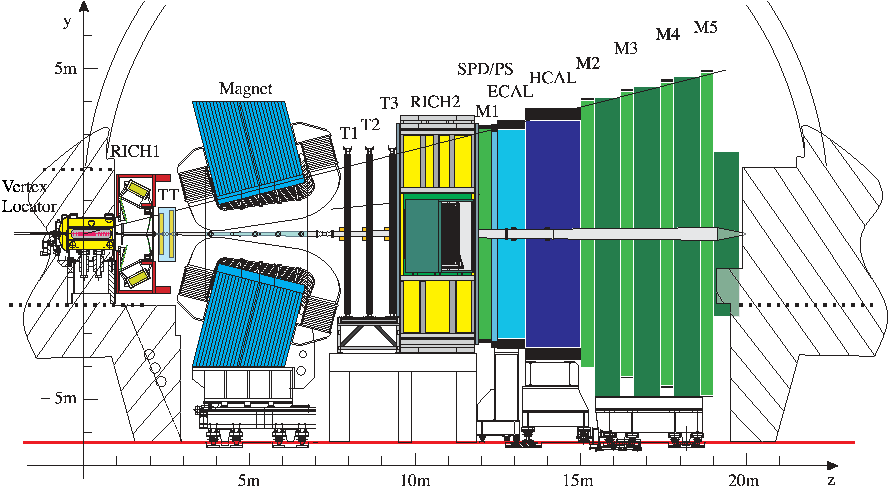
\includegraphics[width=0.8\textheight]{lhcb-detector-cross-section}
%  \caption[Cross-section view of \LHCb, cut in the non-bending $y$--$z$ plane]%
%    {Cross-section view of \LHCb, cut in the non-bending $y$--$z$ plane.}
%  \label{fig:LHCbCrossSection}
%  \end{center}
%\end{sidewaysfigure}



\chapter{Neutrino interactions with atomic nuclei}
\label{chap:NeutrinoInteractionsAtomicNuclei}
The neutrino is a strictly weakly interacting particle.  This has difficult implications for any experiment aiming to study neutrinos as particle detectors generally rely on the electromagnetic force.  In fact, the only proven method of neutrino detection is to utilise a high mass target in which the neutrinos can interact with.  Generally speaking, charged particles are produced by this interaction which can be detected by the usual means.  The collected information from these charged final states can then be used to infer information about the incident neutrino.  All neutrino experiments rely on this method and so any attempted measurements (e.g. $/delta$) rely on our understanding on neutrino interactions with atomic nuclei.  Our understanding of such processes is emcompassed in the models we use to simulate the interactions.

\section{Neutrino interactions at the GeV-scale}
\label{sec:NeutrinoInteractionsGeVScale}
For neutrino energies below $\sim$2~GeV, the neutrino-hadron interactions are largely Quasi-Elastic (QE) [INSERT ZELLER REFERENCE].  In such an interaction, the incident neutrino scatters of the nucleon as if it were a single particle, rather than with one of the nucleon's constituent partons.  As the neutrino is weakly interacting, there are two channels available: the Charge Current (CC) interaction in which are W boson is exchanged and the Neutral Current (NC) interaction in which a Z boson is exchanged.  In the case of a CCQE interaction, the neutrino is converted into its charged lepton equivalent and the target neutron converted to a proton.  In the specific case of an incident $\nu_\mu$, the interaction takes the following form
\begin{equation}
\nu_\mu n \rightarrow \mu^- p
\label{eq:CCQEInteraction}
\end{equation}
For NCQE interactions, the incident neutrino remains after the interaction has occurred and no nucleon coversion takes place.  Because of this fact, the target nucleon in a NCQE interaction need not be a neutron.  So, for $\nu_\mu$ NCQE interactions, there are two channels available
\begin{equation}
\nu_\mu n \rightarrow \nu_\mu n,
\label{eq:NCQEInteractionNeutronTarget}
\end{equation}
\begin{equation}
\nu_\mu p \rightarrow \nu_\mu p
\label{eq:NCQEInteractionProtonTarget}
\end{equation}

